\documentclass[handout]{beamer}
\usetheme{Hannover}
\usecolortheme{dolphin}

\usepackage{tipa}
\usepackage{qtree}
\usepackage{ccicons}
\usepackage{menukeys}
% \usepackage{hyperref}

\title{Praat Scripting Workshop}
\institute{Graduate Linguistics Student Association\\Georgetown University\\jeh241@georgetown.edu}
\author{Jonathan Havenhill}
\date{November 15, 2014}

\begin{document}

\frame{\titlepage
\begin{flushright}\ccbyncsa\end{flushright}}

\frame{\scriptsize\tableofcontents}

\section*{Files for today}
\begin{frame}[fragile]
\frametitle{Files for today}
\begin{itemize}
	\item <1-> You should download the following files:
    \begin{itemize}
	   \item <1-> \url{github.com/jhavenhill/praatscriptingworkshop}
    \end{itemize}

	\item <2-> If you don't have Praat installed, you should download it now:
	\begin{itemize}
		\item <2-> \url{www.fon.hum.uva.nl/praat/}
	\end{itemize}
\end{itemize}

\end{frame}

\section{Introduction}

\begin{frame}[fragile]
\frametitle{Some basic information}

What are the benefits of scripting Praat?\footnote{\scriptsize Adapted from Shigeto Kawahara}

\begin{itemize}
\item <1-> Save time:
\begin{itemize}
    \item Scripting takes a while, but not as long as, say, measuring 800 tokens for 20 variables each
\end{itemize}

\item <2-> Consistency:
\begin{itemize}
    \item Doing things by hand can lead to a lot of mistakes
\end{itemize}

\item <3-> Some things are too difficult or annoying to do by hand:
\begin{itemize}
    \item Calculating vowel midpoints
    \item Measuring formants at F1 maximum
\end{itemize}

\item <4-> It forces you to think about what exactly you're measuring
\end{itemize}
\end{frame}

\begin{frame}[fragile]
\frametitle{Demo: Consistency}

\begin{itemize}
\item <1-> Open ``dutch1.wav''
\item <1-> Get the values of F1 and F2 at the midpoint
\begin{itemize}
    \item What did you get?
\end{itemize}

\item <2-> Scripts require you to be explicit:
\begin{verbatim}
    selectObject ("Sound dutch1")
    do ("To Formant (burg)...", 0, 5, 5500,
     0.025, 50)
    do ("Get value at time...", 1, 0.382,
     "Hertz", "Linear")
\end{verbatim}
\end{itemize}

\end{frame}

\subsection{Tour of Praat}

\begin{frame}[fragile]
\frametitle{Objects Window}
    
\begin{columns}[]
  \begin{column}{0.5\textwidth}
    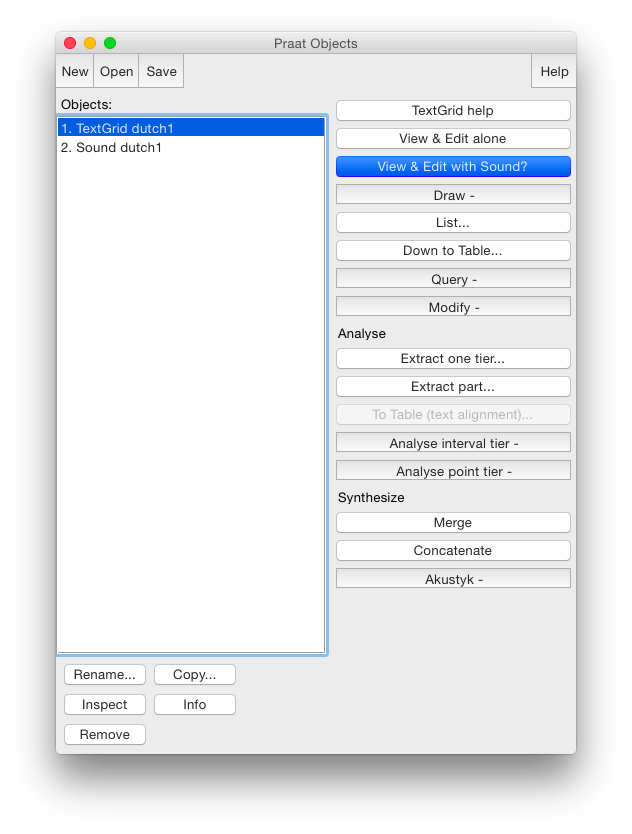
\includegraphics[width=\textwidth]{graphics/objectswindow.png}
  \end{column}

  \begin{column}{0.5\textwidth}
    \begin{itemize}
        \item <1-> This is the main window in Praat
        \item <2-> Every file that you open or create with Praat will appear here
        \item <3-> To apply a script to an Object, you must open it first
    \end{itemize}
  \end{column}
\end{columns}

\end{frame}

\begin{frame}[fragile]
\frametitle{Objects Window}
    
\begin{columns}[]
  \begin{column}{0.5\textwidth}
    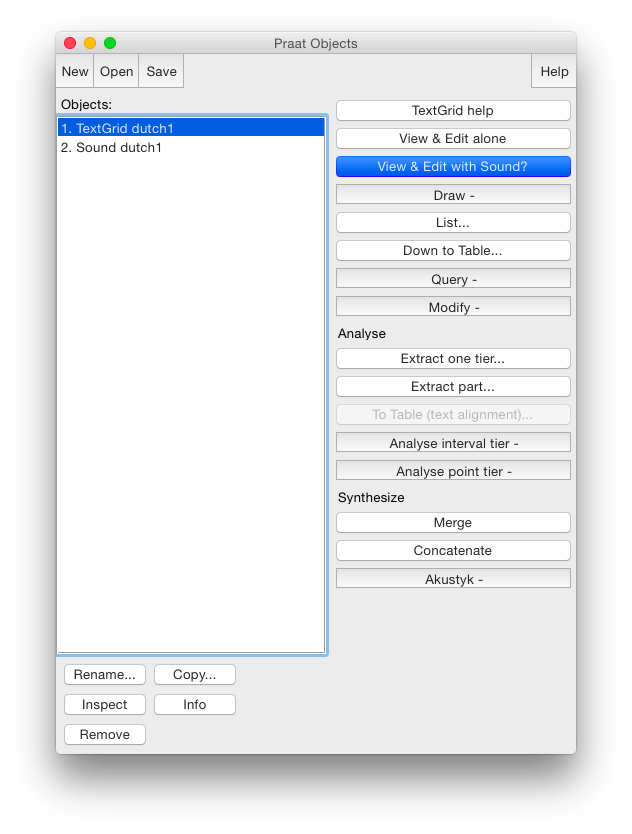
\includegraphics[width=\textwidth]{graphics/objectswindow.png}
  \end{column}

  \begin{column}{0.5\textwidth}
    \begin{itemize}
        \item <1-> There are many types of Object, e.g. Sound and TextGrid
        \item <2-> Each has different actions you can apply to it \begin{itemize}
            \item These appear as dynamic buttons on the right side
        \end{itemize}
        \item <3-> The buttons at the bottom are fixed
    \end{itemize}
  \end{column}
\end{columns}

\end{frame}

\begin{frame}[fragile]
\frametitle{SoundRecorder}
    
\begin{columns}[]
  \begin{column}{0.5\textwidth}
    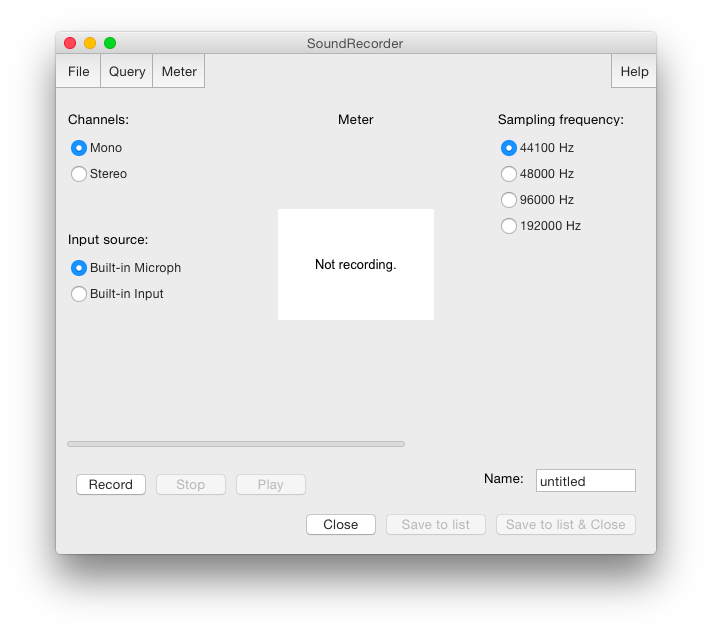
\includegraphics[width=\textwidth]{graphics/soundrecorder.png}
  \end{column}

  \begin{column}{0.5\textwidth}
    \begin{itemize}
        \item <1->\menu{New > Record mono sound\ldots}
        \item <1--> Record yourself saying \textbf{``Hello, World''} in the language of your choice
        \item <2-> Select \menu{Save to list \& Close}
        \item <3-> This saves your sound to the Objects window (but does not save it to disk)
    \end{itemize}
  \end{column}
\end{columns}

\end{frame}

\begin{frame}[fragile]
\frametitle{Editor windows}
    
\begin{columns}[]
  \begin{column}{0.5\textwidth}
    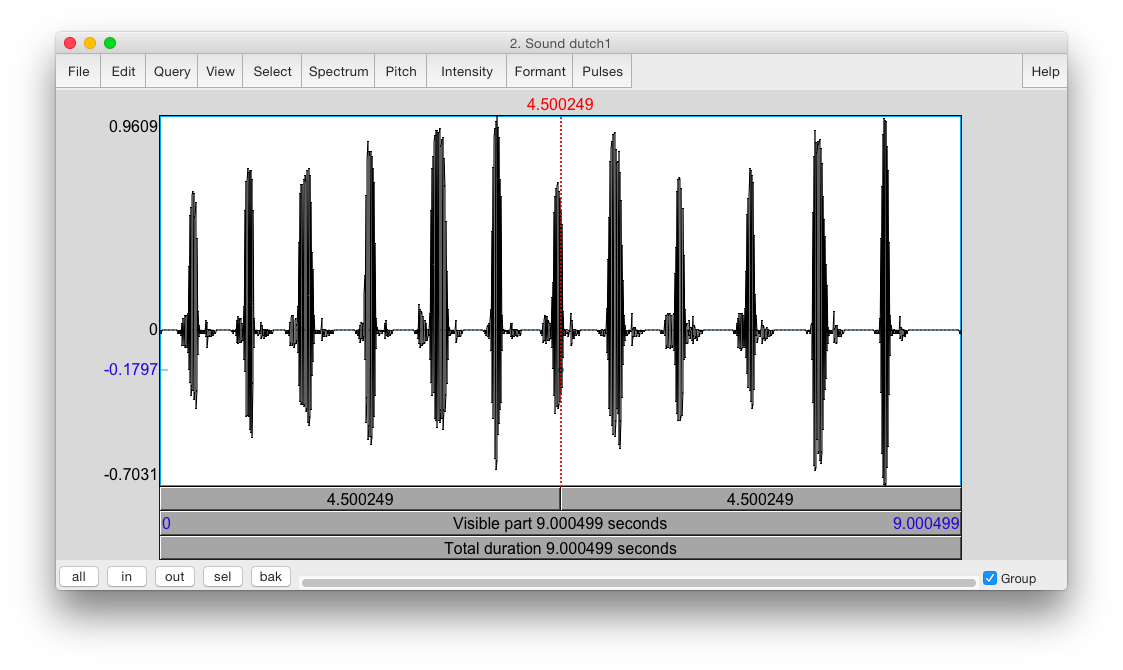
\includegraphics[width=\textwidth]{graphics/editorwindow.png}
  \end{column}

  \begin{column}{0.5\textwidth}
    \begin{itemize}
        \item <1-> Some object types can be opened in an Editor window
        \item <2-> Each has its own, unique Editor window (there are 13 in total)
        \item <3-> You can script Editor functions, but this is generally dispreferred
    \end{itemize}
  \end{column}
\end{columns}

\end{frame}

\begin{frame}[fragile]
\frametitle{Picture window}
    
\begin{columns}[]
  \begin{column}{0.5\textwidth}
    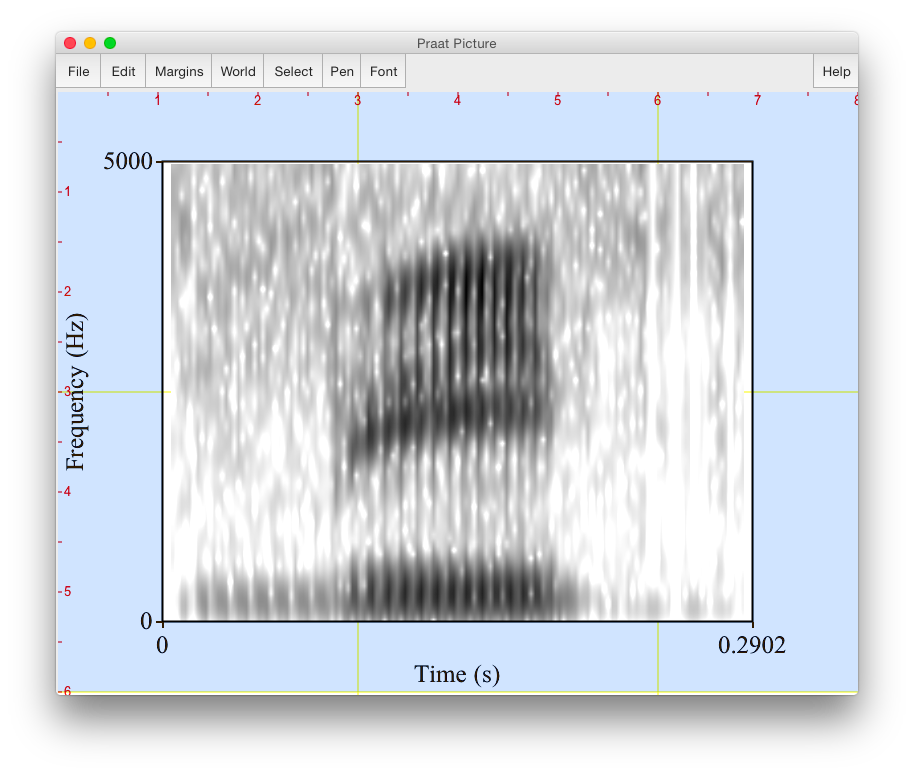
\includegraphics[width=\textwidth]{graphics/picturewindow.png}
  \end{column}

  \begin{column}{0.5\textwidth}
    \begin{itemize}
        \item <1-> This window is actually useful
        \item <2-> You can create high-quality graphs and images for using in your papers (much better than screenshots of the Editor window)
    \end{itemize}
  \end{column}
\end{columns}
\end{frame}

\begin{frame}[fragile]
\frametitle{Picture window demo}
    \begin{itemize}
        \item <1-> First, draw a Spectrogram of the sound you recorded:
        \begin{itemize}
            \item Select Sound in Objects window
            \item \menu{Analyze Spectrum > To Spectrogram... > OK}
            \item Select Spectrogram in Objects window
            \item \menu{Draw > Paint > OK}
        \end{itemize}
        \item <1-> Then, try playing around with some of the functions in the ``World'' menu (use \keys{\cmd/Ctrl + E} to start over)
    \end{itemize}
\end{frame} 

\begin{frame}[fragile]
\frametitle{Finally: the ScriptEditor}
    
\begin{columns}[]
  \begin{column}{0.5\textwidth}
    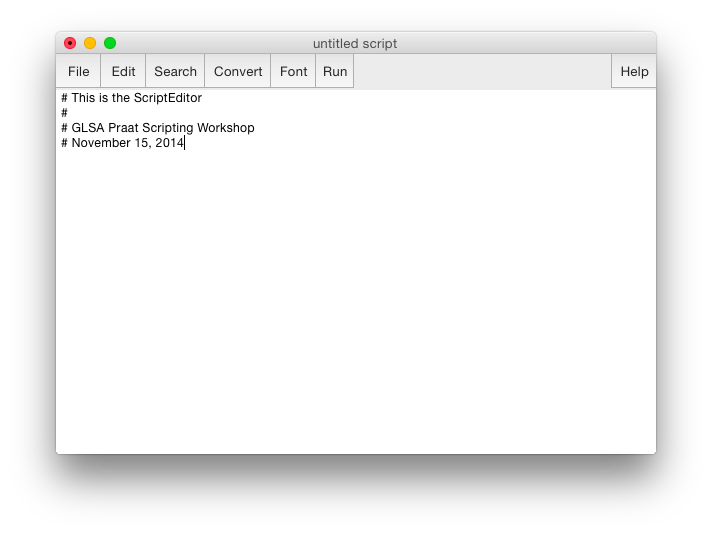
\includegraphics[width=\textwidth]{graphics/scripteditor.png}
  \end{column}

  \begin{column}{0.5\textwidth}
    \begin{itemize}
        \item <1-> \menu{Praat > New Praat script}
        \item <2-> Once you start writing complex scripts, you'll probably want to use an editor made for coding
        \item <3-> But you'll always need the ScriptEditor for two important features\ldots
    \end{itemize}
  \end{column}
\end{columns}

\end{frame}

\begin{frame}[fragile]
\frametitle{ScriptEditor}
    
\begin{columns}[]
  \begin{column}{0.5\textwidth}
    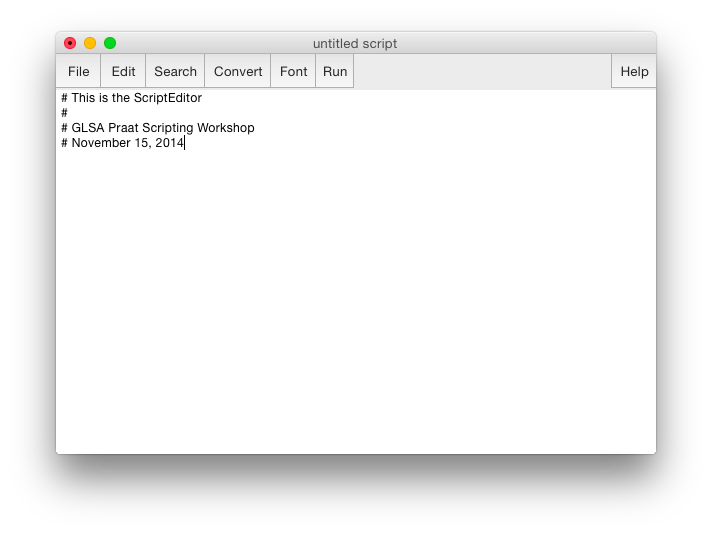
\includegraphics[width=\textwidth]{graphics/scripteditor.png}
  \end{column}

  \begin{column}{0.5\textwidth}
    \begin{itemize}
        \item <1-> Run and Run Selection 
        \begin{itemize}
            \item Run: \keys{\cmd/Ctrl + R}
            \item Run selection: \keys{\cmd/Ctrl + T}
        \end{itemize}
        \item <2-> Command History
        \begin{itemize}
            \item \menu{Edit > Paste history}
            \item \keys{\cmd/Ctrl + H}
        \end{itemize}
    \end{itemize}
  \end{column}
\end{columns}

\end{frame}

% !!! Insert selectObject exercise here

\begin{frame}[fragile]
\frametitle{Exercise}
\begin{itemize}
    \item First, save the ``Hello World'' sound you recorded to somewhere on your computer
    \item Then, write a script that does the following:
    \begin{itemize}
        \item Read the .wav from disk
        \item Paint a spectrogram of the sound in the Picture window, showing 0-8000 Hz.
    \end{itemize}
    Bonus:
    \begin{itemize}
        \item Give the spectrogram dimensions of 4 in x 6 in\\(hint: size is determined by the viewport)
        \item Give your Spectrogram a title like ``Hello World''\\(hint: you want the title to go in the margin)
        \item Save your Spectrogram as a PDF
    \end{itemize}
\end{itemize}
\end{frame}

\section{The Basics}

\begin{frame}[fragile]
\frametitle{One more: the Info window}

\begin{columns}[]
    \begin{column}{0.5\textwidth}
        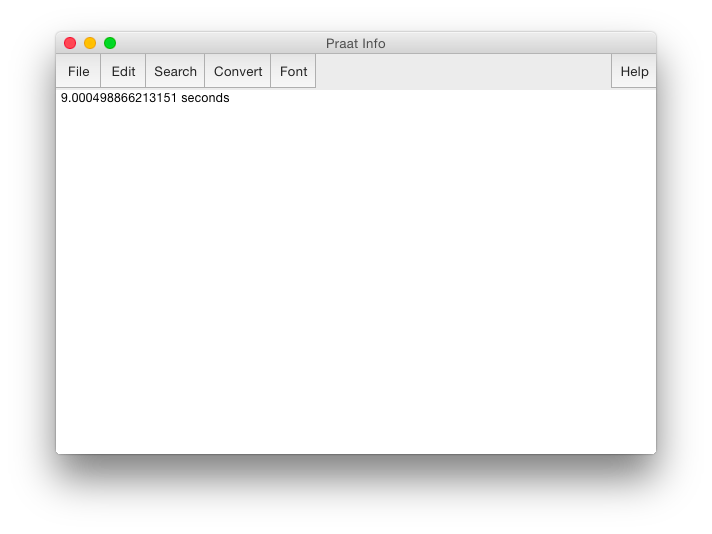
\includegraphics[width=\textwidth]{graphics/infowindow.png}
    \end{column}

    \begin{column}{0.5\textwidth}
        \begin{itemize}
            \item <1-> The Info window displays...info!
            \item <2-> This is the window that pops up when you take formant measurements
            \item <2-> But you can write things to it as well
        \end{itemize}
    \end{column}
\end{columns}
\end{frame}

\begin{frame}[fragile]
\frametitle{Info window}
\begin{itemize}
    \item <1-> Type the following into the ScriptEditor:
    \begin{verbatim}
    writeInfoLine ("Hello, world!")\end{verbatim}
    \item <1-> Click \menu{Run > Run}

    \item <2-> Now, try adding another line:
    \begin{verbatim}
    writeInfoLine ("Hello, world!")
    writeInfoLine ("How art thou?")\end{verbatim}
    \item <2-> What happens?
\end{itemize}
\end{frame}

\begin{frame}[fragile]
\frametitle{Info window}
\begin{itemize}
    \item <1-> We need another command:
    \begin{verbatim}
    writeInfoLine ("Hello, world!")
    appendInfoLine ("How art thou?")\end{verbatim}

    \item <1-> \texttt{writeInfoLine} erases the contents of the Info window before printing, \texttt{appendInfoLine} doesn't
\end{itemize}
\end{frame}

\begin{frame}[fragile]
\frametitle{Comments}
\begin{itemize}
    \item <1-> It's important to comment your code, so others (and Future You) will know how it works
    \item <2-> Comments in Praat start with \texttt{\#} or \texttt{;} (semicolon):
    \begin{verbatim}
    # This is a comment
    ; This is also a comment\end{verbatim}
    \item <3-> Comments starting with \texttt{\#} can be used inline, while comments starting with \texttt{;} cannot
    \item <4-> It's also a good idea to leave a blurb at the beginning of your script that explains what it does and who wrote it:
    \begin{verbatim}
    # This script extracts formants
    # and vowel duration and saves
    # the values to a .csv
    #
    # Jon Havenhill - 15 Nov 2014
    \end{verbatim}
\end{itemize}
\end{frame}

\begin{frame}[fragile]
\frametitle{White Space}
\begin{itemize}
    \item <1-> Praat doesn't care about white space, unlike some other languages (such as Python)
    \item <1-> However, it is good practice to indent your code:
    \begin{verbatim}
    for i from 1 to 10
        do (...)
        for j from 2 to 20
            do (...)
        endfor
    endfor
    \end{verbatim}

    \item <2-> Four spaces for each level is customary
    \item <2-> Praat also ignores blank lines, so you can use them to visually organize your code  
\end{itemize}
\end{frame}

\begin{frame}[fragile]
\frametitle{Long lines}
\begin{itemize}
    \item <1-> Sometimes lines get really long:
    \begin{verbatim}appendInfoLine("analyzeFilesResults.txt", "dialect",
tab$, "subject", tab$, "real", tab$,
"consonant", tab$, "following vowel",
tab$, "notes", tab$, "repetition",
tab$, "word", tab$, "environment", tab$,
"dur preceding V", tab$, "dur preceding N",
tab$, "closure dur", tab$, "voicing dur",
tab$, "vowel intensity", tab$, "VOT", tab$, "frication", tab$, "F0 into closure", tab$,
"F1 into closure", tab$, "F0 out of closure",
tab$, "F1 out of closure") 
    \end{verbatim}

    \item <2-> So you can break them up with an ellipsis (\texttt{...})
    \begin{verbatim}Create Sound from formula: "windowedSine", 1, 0, 1, 44100,
... "0.5 * sin(2*pi*1000*x) * exp(-0.5*((x-0.5)/0.1)^2)"
\end{verbatim}
\end{itemize}
\end{frame}

\subsection{Numeric variables}

\begin{frame}[fragile]
\frametitle{Variables}
\begin{itemize}
    \item <1-> Variables allow you to store some piece of information in memory for later use
    \item <2-> Praat has two kinds:
    \begin{itemize}
        \item Numeric variables
        \item String variables
    \end{itemize}
    \item<3-> Variable names must start with a lower-case letter, but they may contain capital letters, numbers, or underscores:
    \begin{columns}[]
        \begin{column}{0.5\textwidth}
            \begin{verbatim}
            formant
            formant1
            f1
            f1_max
            \end{verbatim}
        \end{column}

        \begin{column}{0.5\textwidth}
            not: \texttt{Formant}\\
            not: \texttt{formant!}\\
            not: \texttt{F1}\\
            not: \texttt{f1-max}
        \end{column}
    \end{columns}
\end{itemize}
\end{frame}

\begin{frame}[fragile]
\frametitle{Numeric Variables}
\begin{itemize}
    \item <1-> Numeric variables may contain integers or decimal (real) numbers
    \item <1-> Values less than 1 must have a preceding 0
    \begin{itemize}
        \item \texttt{0.5} \emph{not} \texttt{.5}
    \end{itemize}
    \item <1-> Variables are assigned using the equal sign:
    \begin{verbatim}
    formant = 1500
    writeInfoLine ("The formant value is: ",
    ... formant, ".")
    \end{verbatim}

    \item <2-> What will this give us?
    \begin{verbatim}
    formant = 1500
    formant = 1650
    writeInfoLine ("The formant value is: ",
    ... formant, ".")
    \end{verbatim}
\end{itemize}
\end{frame}

\begin{frame}[fragile]
\frametitle{Numeric Variables}
\begin{itemize}
    \item <1-> Variables may also contain other variables:
    \begin{verbatim}
    formant1 = 500
    formant2 = formant1 * 2
    writeInfoLine ("F1 is half of: ",
    ... formant2, ".")
    \end{verbatim}

    \item <2-> What will this give us?
    \begin{verbatim}
    b = 3.1
    c = b * 2
    b = 5.8
    writeInfoLine ("The value of c is ", c, ".")
    \end{verbatim}

    \item <3-> It gives us \textbf{6.2}, not \textbf{11.6}. \texttt{c} is assigned the value of \texttt{b} at the moment of evaluation
\end{itemize}
\end{frame}

\begin{frame}[fragile]
\frametitle{Numeric Operators}
\begin{itemize}
    \item <1-> Math:
    \begin{itemize}
        \item Negation: \texttt{-}
        \item Exponentiation: \texttt{\^}
        \item Multiplication: \texttt{*}
        \item Division: \texttt{/}
        \item Addition: \texttt{+}
        \item Subtraction: \texttt{-}
    \end{itemize}

    \item <2-> Integer division (same precedence as \texttt{*} and \texttt{/}):
    \begin{itemize}
        \item \texttt{div}: division rounded down
        \item \texttt{mod}: the remainder
    \end{itemize}

    \item <3-> What do the following operations give us?
    \begin{verbatim}
    f0 = 188
    a = f0 div 10
    b = f0 mod 10
    writeInfoLine ("The value of a is ", a, ".")
    appendInfoLine ("The value of b is ", b, ".")
    \end{verbatim}
\end{itemize}
\end{frame}

\begin{frame}[fragile]
\frametitle{Numeric Variables}
\begin{itemize}
    \item <1-> Constants:
    \begin{itemize}
        \item \texttt{pi} ($\pi$)
        \item \texttt{e} ($e$)
        \item (You can't use these as names of variables)
    \end{itemize}

    \item <2-> Functions:
    \begin{itemize}
        \item Convert to string (and back):
        \begin{verbatim}f0$ = string$ (f0)
f0 = number (f0$)
        \end{verbatim}

        \item Round to $n$ decimal places:
        \begin{verbatim}f0 = 233.23792719
writeInfoLine ("The F0 is: ", fixed$(f0, 2),
... " Hz.")
        \end{verbatim}

        \item Display as percentage with $n$ decimal places:
        \begin{verbatim}score = 87.3 / 100
writeInfoLine ("Your score is: ",
... percent$(score, 2))
        \end{verbatim}
    \end{itemize}
\end{itemize}
\end{frame}

\subsection{String variables}

\begin{frame}[fragile]
\frametitle{String Variables}
\begin{itemize}
    \item <1-> String variables must end with a dollar sign (`\texttt{\$}')
    \begin{verbatim}
    helloworld$ = "Hello, World!"
    \end{verbatim}

    \item <1-> When assigning a value to a string variable, the string must be enclosed in double quotation marks

    \item <1-> Can be empty: \texttt{empty\$ = ""}
\end{itemize}
\end{frame}

\begin{frame}[fragile]
\frametitle{Concatenation/Truncation}
\begin{itemize}
    \item <1-> Like numeric variables, string variables have operators:
    \begin{itemize}
        \item Concatenate: \texttt{a\$ + b\$}
        \item Truncate: \texttt{a\$ - b\$}
    \end{itemize}

    \begin{verbatim}
    fileName$ = "vowels.wav"
    tgName$ = fileName$ - ".wav" + ".TextGrid"
    writeInfoLine("The name of the TextGrid
    ... is: ", tgName$)
    \end{verbatim}

    \item<3-> What happens if the file is a \texttt{.aiff}?
    \begin{verbatim}
    fileName$ = "vowels.aiff"
    tgName$ = fileName$ - ".wav" + ".TextGrid"
    writeInfoLine("The name of the TextGrid
    ... is: ", tgName$)
    \end{verbatim}

\end{itemize}
\end{frame}

\begin{frame}[fragile]
\frametitle{String Functions}
\begin{itemize}
    \item <1-> There are also a number of functions that can be used with strings

    \item <1-> Some return strings, others numbers
    \begin{itemize}
        \item \texttt{length (string\$)}
        \item \texttt{number (string\$)}
    \end{itemize}

    \begin{verbatim}
    word$ = "exquisite"
    wordLength = length (word$)
    writeInfoLine("There are ", wordLength,
    ... " characters in ", word$)
    \end{verbatim}

    \begin{verbatim}
    string$ = "5e6"
    value = number (string$) * 2
    writeInfoLine("The value is: ", value)
    \end{verbatim}

\end{itemize}
\end{frame}

\begin{frame}[fragile]
\frametitle{String Functions}
\begin{itemize}
    \item <1-> Extracting parts of strings:
    \begin{itemize}
        \item \texttt{left\$ (string\$, n)}
        \item \texttt{right\$ (string\$, n)}
        \item \texttt{mid\$ (string\$, n, m)}
    \end{itemize}

    \begin{verbatim}
    word$ = "working"
    wordEnding$ = right$ (word$, 3)
    wordStem$ = left$ (word$, 4)
    writeInfoLine("The suffix is: ",
    ... wordEnding$)
    appendInfoLine("The stem is: ", wordStem$)
    \end{verbatim}

    \begin{verbatim}
    word$ = "working"
    preceding$ = mid$ (word$, 4, 1)
    writeInfoLine("The preceding segment is: ",
    ... preceding$)
    \end{verbatim}

\end{itemize}
\end{frame}

\begin{frame}[fragile]
\frametitle{String Functions}
\begin{itemize}
    \item <1-> Extracting parts of strings:
    \begin{itemize}
        \item \texttt{index (stringA\$, stringB\$)}:
        \\Finds first occurrence of \emph{stringB\$} in \emph{stringA\$}
        \item \texttt{rindex (stringA\$, stringB\$)}:
        \\Finds last occurrence
    \end{itemize}

    \begin{verbatim}
    word$ = "working"
    vowel$ = "i"
    first = index (word$, vowel$)
    writeInfoLine("The first occurrence of ""i""
    ... is the ", first, "th character")
    \end{verbatim}

    \item <1-> NB: the index starts at 1, not at 0 like in some other languages

\end{itemize}
\end{frame}

\begin{frame}[fragile]
\frametitle{String Functions}
\begin{itemize}
    \item <1-> Searching strings:
    \begin{itemize}
        \item \texttt{startsWith (stringA\$, stringB\$)}
        \item \texttt{endsWith (stringA\$, stringB\$)}
    \end{itemize}
    Retuns 1 if true, 0 if false

    \begin{verbatim}
    word$ = "working"
    suffix$ = "ing"
    value = endsWith (word$, suffix$)
    writeInfoLine("This word ends in ""ing"": ",
    ... value)
    \end{verbatim}

\end{itemize}
\end{frame}

\begin{frame}[fragile]
\frametitle{String Functions}
\begin{itemize}
    \item <1-> Replace:
    \begin{itemize}
        \item \texttt{replace\$ (stringA\$, stringB\$, stringC\$, n)}
    \end{itemize}
    \item <1-> Returns a string \emph{like} \texttt{stringA\$}, but where \texttt{stringB\$} has been replaced with \texttt{stringC\$} $n$ times.

    \begin{verbatim}
    word$ = "working"
    suffix$ = "ing"
    newSuffix$ = "ed"
    newWord$ = replace$ (word$, suffix$,
    ... newSuffix$, 1)
    writeInfoLine("The new word is: ",
    ... newWord$)
    \end{verbatim}

\end{itemize}
\end{frame}

\begin{frame}[fragile]
\frametitle{Predefined Variables}
\begin{itemize}
    \item <1-> \texttt{praatVersion}: Current version of Praat (e.g. 5401)
    \item <1-> \texttt{macintosh}/\texttt{windows}/\texttt{unix}: value of 1 if script is running on that platform
    \item <1-> \texttt{defaultDirectory\$}: Directory in which the script is saved

    \item <2-> \texttt{newline\$}: Inserts a linebreak
    \item <2-> \texttt{tab\$}: Inserts a tab

    \begin{verbatim}
    f1 = 650
    f2 = 1500
    newSuffix$ = "ed"
    writeInfoLine("F1 is ", f1, " Hz.",
    ... newline$, "F2 is", f2, " Hz.")
    \end{verbatim}

\end{itemize}
\end{frame}

\subsection{Conditionals}

\begin{frame}[fragile]
\frametitle{Operators}
\begin{itemize}
    \item <1-> In addition to mathematical operations, there are comparison operators:
    \begin{itemize}
        \item \texttt{=}\phantom{>>} equal
        \item \texttt{<>}\phantom{>} does not equal
        \item \texttt{<}\phantom{>>} less than
        \item \texttt{>}\phantom{>>} greater than
        \item \texttt{<=}\phantom{>} less than or equal
        \item \texttt{>=}\phantom{>} greater than or equal
    \end{itemize}

    \item <1-> You'll need these for conditionals and \texttt{while} loops

    \item <2-> Some comparison operators from other languages can be used, for example \texttt{==} for equal and \texttt{!=} for unequal

    \item <2-> Comparison operations return a value of 0 (if false) or 1 (if true)---these values can be saved to a variable

\end{itemize}
\end{frame}

\begin{frame}[fragile]
\frametitle{Operators}
\begin{itemize}
    \item <1-> Comparison operators can also be used with string variables:
    \begin{itemize}
        \item \texttt{a\$ = b\$}: true if strings are equal
        \item \texttt{a\$ <> b\$}: true if strings are unequal
    \end{itemize}
    \item <2-> These are a bit less intuitive:
    \begin{itemize}
        \item \texttt{a\$ < b\$}: true if \texttt{a\$} precedes \texttt{b\$} in ASCII sorting order
        \item \texttt{a\$ > b\$}: true if \texttt{b\$} precedes \texttt{a\$}
        \item \texttt{a\$ <= b\$}: true if \texttt{a\$} precedes or is equal to \texttt{b\$}
        \item \texttt{a\$ >= b\$}: true if \texttt{b\$} precedes or is equal to \texttt{a\$}
    \end{itemize}

    \item <3-> ASCII sorting order:
    \begin{itemize}
        \item Numbers precede letters
        \item Capital letters precede lower case letters
        \item Numbers are sorted by their individual characters, e.g., 10 comes before 2 
    \end{itemize}

\end{itemize}
\end{frame}

\begin{frame}[fragile]
\frametitle{Conditionals}
\begin{itemize}
    \item <1-> \texttt{if}: introduces conditional
    \item <1-> \texttt{elsif}: introduces possible alternate outcome
    \item <1-> \texttt{else}: executed if none of the preceding tests were true
    \item <1-> \texttt{endif}: ends conditional
    
    \begin{verbatim}
    if x = y
        do something
    elsif x = z
        do something else
    else
        do yet another thing
    endif
    \end{verbatim}

    \item <1-> \scriptsize NB: It's much easier to read if you indent, but it's not strictly necessary. But use spaces, not tabs. Tabs are rendered inconsistently across text editors.

\end{itemize}
\end{frame}

\begin{frame}[fragile]
\frametitle{Conditionals}
\begin{itemize}
    \item <1-> Logical operators:
    \begin{itemize}
        \item not
        \item and
        \item or
    \end{itemize}
    
    \begin{verbatim}
    if ((x = y) and (x = w))
        do something
    elsif ((x = z) or (x = q))
        do something else
    elsif ((x = s) and not (x = t))
        do something else
    else
        do yet another thing
    endif
    \end{verbatim}

    \item <1-> \texttt{not} takes precedence over \texttt{and}, which takes precedence over \texttt{or}. But it's easier if you just use parentheses.

\end{itemize}
\end{frame}

\begin{frame}[fragile]
\frametitle{Conditionals}
\begin{itemize}
    \item <1-> Let's write one together
    \begin{itemize}
        \item Generate a random number from 1 to 100
        \item Test whether number is greater than 50
        \item Write the results to the Info line
    \end{itemize}
    
    \item<2->
    \begin{verbatim}
    number = randomInteger(1, 100)

    if number > 50
        writeInfoLine ("The number was 
        ... greater than 50.")
    elsif number = 50
        writeInfoLine ("The number was 50.")
    else
        writeInfoLine ("The number was
        ... less than 50.")
    endif
    \end{verbatim}

\end{itemize}
\end{frame}

% \begin{frame}[fragile]
% \frametitle{Conditionals}
% \begin{itemize}
%     \item <1-> Let's make it more complicated
%     \begin{itemize}
%         \item Test for the values of two numbers
%     \end{itemize}
    
%     \item<2->
%     \begin{verbatim}
%     number = randomInteger(1, 100)

%     if number > 50
%         writeInfoLine ("The number was 
%         ... greater than 50.")
%     elsif number = 50
%         writeInfoLine ("The number was 50.")
%     else
%         writeInfoLine ("The number was
%         ... less than 50.")
%     endif
%     \end{verbatim}

% \end{itemize}
% \end{frame}

\begin{frame}[fragile]
\frametitle{Exercise: Variables and Conditionals}
\begin{itemize}
    \item Write a script to determine whether a given year is a leap year
    \item Leap years occur every 4 years, unless the year is divisible by 100. Years divisible by 400 are leap years as well.
    \item Write the results to the Info window
    \item Hint: If a year is divisible by 4, its remainder will be 0
    \item Bonus:
    \begin{itemize}
        \item Prompt the user for the year (see \url{http://www.fon.hum.uva.nl/praat/manual/Scripting_6_1__Arguments_to_the_script.html})
        \item Prompt the user for a date in some format, like 11/15/2014 or November 2014, then determine whether that date is in a leap year
    \end{itemize}
\end{itemize}
\end{frame}

\begin{frame}[fragile]
\frametitle{Exercise: Basic Solution}
    
\begin{verbatim}
year = 2004

if (((year mod 4 == 0) and (year mod 100 <> 0))
... or (year mod 400 == 0))
    writeInfoLine (year, "is a leap year!")
else
    writeInfoLine (year, "is not a leap year!")
endif
\end{verbatim}

\end{frame}

\begin{frame}[fragile]
\frametitle{Exercise: Bonus Solution}

\begin{verbatim}
form Give me a year:
    integer year
endform

if (((year mod 4 == 0) and (year mod 100 <> 0))
... or (year mod 400 == 0))
    writeInfoLine (year, "is a leap year!")
else
    writeInfoLine (year, "is not a leap year!")
endif
\end{verbatim}
\end{frame}

\begin{frame}[fragile]
\frametitle{Exercise: Bonus Solution 2}

\begin{verbatim}
form Give me a date:
    text date
endform
index = index_regex(date$, "[0-9][0-9][0-9][0-9]")
if index <> 0
    year = number (mid$ (date$, index, 4))
    if (((year mod 4 == 0) and (year mod 100 <> 0))
    ... or (year mod 400 == 0))
        writeInfoLine (year, " is a leap year!")
    else
        writeInfoLine (year, " is not a leap year!")
    endif
else
    writeInfoLine ("Please enter a date with
    ... a 4-digit year.")
endif
\end{verbatim}
\end{frame}

\begin{frame}[fragile]
\frametitle{Review}


\end{frame}

\section{Loops}

\begin{frame}[fragile]
\frametitle{Loops}

\begin{itemize}
    \item <1-> The best reason to script Praat---taking care of mundane, repetitive tasks
    \item <1-> A loop is a set of commands that is repeated until some condition is met
    \item <1-> There are three basic types of loop in Praat:
    \begin{itemize}
        \item For loop
        \item While loop
        \item Until loop
    \end{itemize}
\end{itemize}  
\end{frame}

\subsection{For Loops}

\begin{frame}[fragile]
\frametitle{For Loops}

\begin{itemize}
    \item <1-> A for loop is a loop which repeats a given number of times

    \item <1-> A skeleton for loop:
    \begin{verbatim}
    for i from x to y
        do something
    endfor
    \end{verbatim}

    \item <2-> The statement between \texttt{for} and \texttt{endfor} is executed, and \texttt{i} increases by 1 each time

    \item <3-> The \texttt{from x} statement is optional. If you don't include it, \texttt{i} starts at 1    

\end{itemize}  
\end{frame}

\begin{frame}[fragile]
\frametitle{For Loops}

\begin{itemize}
    \item <1-> Plot points to the picture window

    \begin{verbatim}
    do ("Erase all")
    do ("Axes...", 0, 100, 0, 100)
    m = 2
    b = 3
    for x from 1 to 100
        y = m * x + b
        do ("Draw circle...", x, y, 1)
    endfor
    \end{verbatim}

\end{itemize}  
\end{frame}

\begin{frame}[fragile]
\frametitle{Exercise: For Loops}

\begin{itemize}
    \item <1-> Let's make a loop that simulates a coin toss
    \item <1-> Use a for loop to:
    \begin{itemize}
        \item Generate a random integer ``between'' 1 and 2
        \item Use an if statement to save the result as either a heads or tails
        \item Repeat 100 times
        \item Write the results to the Info window
    \end{itemize}

\end{itemize}  
\end{frame}

\begin{frame}[fragile]
\frametitle{Solution: Coin Toss}
\begin{verbatim}
    heads = 0
    tails = 0
    for toss from 1 to 100
        flip = randomInteger(0, 1)
        if flip = 0
            heads = heads + 1
        else
            tails = tails + 1
        endif
    endfor
    writeInfoLine ("Heads: ", heads,
    ... newline$, "Tails: ", tails)
\end{verbatim}

\end{frame}

\subsection{Until Loops}

\begin{frame}[fragile]
\frametitle{Until Loops}

\begin{itemize}
    \item <1-> An until loop is one which repeats an infinite number of times until some condition is met

    \item <1-> A skeleton until loop:
    \begin{verbatim}
    repeat
        do something
    until x = y
    \end{verbatim}

    \item <2-> The statement will always be completed at least once.
    \begin{itemize}
        \item Try the following. Clear your Info window first with \menu{File > Clear}.
        \begin{verbatim}
        x = 7
        repeat
            appendInfoLine ("test")
        until x > 1
    \end{verbatim}
    \end{itemize}

    \item <3-> The reason why is intuitive: the test isn't conducted until after the first iteration.

\end{itemize}  
\end{frame}

\begin{frame}[fragile]
\frametitle{Until Loops}

\begin{itemize}
    \item <1-> Let's write an until loop

    \item <1-> This script will measure the number of tries it takes to roll 12 with two dice.

    \begin{verbatim}
    throws = 0
    repeat
        roll = randomInteger (1,6) 
        ... + randomInteger (1,6)
        throws = throws + 1
    until roll = 12
    writeInfoLine ("It took ", throws, " throws
    ... to roll 12 with two dice.")
    \end{verbatim}

\end{itemize}  
\end{frame}

\subsection{While Loops}

\begin{frame}[fragile]
\frametitle{While Loops}

\begin{itemize}
    \item <1-> A while loop repeats until some condition no longer holds true

    \item <1-> A skeleton while loop:
    \begin{verbatim}
    while x = y
        do something
    endwhile
    \end{verbatim}

    \item <2-> Unlike until loops, while loops may execute zero times.
    \begin{itemize}
        \item Let's return to the previous example. Again, clear your Info window first using \menu{File > Clear}.
        \begin{verbatim}
        x = 7
        while x < 1
            appendInfoLine ("test")
        endwhile
    \end{verbatim}
    \end{itemize}

    \item <3-> Nothing happens. What would happen if the test was \texttt{while x > 1}?

\end{itemize}  
\end{frame}

\begin{frame}[fragile]
\frametitle{While Loops}

\begin{itemize}
    \item <1-> Let's convert our dice roll script to use a while loop. What do we need to change?

    \item <2-> 
    \begin{verbatim}
    throws = 0
    roll = 0
    while roll <> 12
        roll = randomInteger (1,6) 
        ... + randomInteger (1,6)
        throws = throws + 1
    endwhile
    writeInfoLine ("It took ", throws, " throws
    ... to roll 12 with two dice.")
    \end{verbatim}

\end{itemize}  
\end{frame}

\begin{frame}[fragile]
\frametitle{While Loops vs. Until Loops}

\begin{itemize}
    \item <1-> While loops and until loops are very similar

    \item <2-> Choosing one is really a matter of preference, and whichever is best suited for a specific application

\end{itemize}  
\end{frame}

\begin{frame}[fragile]
\frametitle{Exercise: Nested loops}

\begin{itemize}
    \item <1-> Let's write a script to find all the prime numbers less than $n$
    \begin{itemize}
        \item Use a loop to iterate through each number $x$ to $n$
        \item Use a nested loop to iterate through each possible divisor ($y$) of $x$
        \item Test whether $x$ is evenly divisible by $y$
        \item If $y$ is prime, print it to the Info window
    \end{itemize}

\end{itemize}  
\end{frame}

\begin{frame}[fragile]
\frametitle{Solution: Nested loops}
\begin{verbatim}
max = 100
x = 1
while x < max
x += 1
not_prime = 0
for y from 2 to x-1
    if x mod y = 0
        not_prime += 1
    endif
endfor
if not_prime = 0
    appendInfoLine(x, " is a prime number!")
endif
endwhile
\end{verbatim}
\end{frame}

\section{TextGrids}
\subsection{Structure}

\begin{frame}[fragile]
\frametitle{TextGrids}

\begin{itemize}
    \item <1-> What is a TextGrid, anyway?
    \item <2-> It's really just a text file:
    \scriptsize
    \begin{verbatim}
    File type = "ooTextFile"
    Object class = "TextGrid"

    xmin = 0 
    xmax = 79.79486052387188 
    tiers? <exists> 
    size = 4 
    item []: 
        item [1]:
            class = "IntervalTier" 
            name = "Phrase" 
            xmin = 0 
            xmax = 79.79486052387188 
            intervals: size = 41 
            intervals [1]:
                xmin = 0 
                xmax = 0.7365941687547206 
                text = "" 
            intervals [2]:
                xmin = 0.7365941687547206 
                xmax = 2.2336095443531008 
                text = "say feet again" 
            intervals [3]:
                xmin = 2.2336095443531008 
                xmax = 4.591058605391538 
                text = "" 
            intervals [4]:
                xmin = 4.591058605391538 
                xmax = 6.162924749769843 
                text = "say juice again" 
    \end{verbatim}
\end{itemize}
\end{frame}

\begin{frame}[fragile]
\frametitle{TextGrids}

\begin{itemize}
    \item <1-> What is a TextGrid, anyway?
    \item <1-> It's really just a text file.
    \item <1-> It contains attributes you can extract, either through the dynamic buttons in the Object window, or through a script.

    \item <2-> These attributes include:
    \begin{itemize}
        \item A start time
        \item A stop time
        \item Tiers
    \end{itemize}

    \item <3-> A tier can be an IntervalTier, which contains a set of intervals, each with its own start and stop time

    \item <3-> Or it can be a point tier, just a labeled point in time
\end{itemize}
\end{frame}

\begin{frame}[fragile]
\frametitle{TextGrids}

\begin{itemize}
    \item <1-> TextGrids are perhaps the most useful thing you can script
    \item <1-> You can easily automate extracting any measurement you would take by hand
    \item <2-> And some measurements that are tedious to take by hand, e.g., measuring formants at the point of F1 maximum

\end{itemize}
\end{frame}

\subsection{Creating}

\begin{frame}[fragile]
\frametitle{TextGrids}

\begin{itemize}
    \item <1-> Let's create a TextGrid, first by hand, then using a script.

    \item <1-> Open the ``Hello World'' sound you recorded earlier, or create a new one.

    \item <1-> Create a new TextGrid with \menu{Annotate > To TextGrid...} 

    \item <1-> Name the tiers: \texttt{words}, \texttt{vowels}, and \texttt{midpoints}. Make \texttt{midpoints} be a point tier

    \item <2-> Now, open the ScriptEditor and paste your command history
    \begin{verbatim}
    selectObject ("Sound helloworld")
    do ("To TextGrid...", "words vowels
    ... midpoints", "midpoints")
    \end{verbatim}

    \item <3-> Tier names are given in a space-delimited string of names

\end{itemize}
\end{frame}

\begin{frame}[fragile]
\frametitle{Practice: Working with TextGrids}

\begin{itemize}
    \item <1-> Annotate your ``Hello, World'' file
    \vspace{\baselineskip}
    \item <1-> Start with the words tier. Click the point where the word starts, and choose \menu{Boundary > Add on tier 1}
    \item <1-> Do the same at the point where the word ends.
    \item <1-> Click between the boundaries and type a label
    \item <1-> Repeat for each word and vowel
    \item <1-> Save as a text file \menu{File > Save TextGrid as text file...}\\or \keys{\cmd/Ctrl + S}
\end{itemize}
\end{frame}

\begin{frame}[fragile]
\frametitle{Practice: Working with TextGrids}

\begin{itemize}
    \item <1-> Okay, now let's write a basic script to extract some measurements

    \item <1-> Get the duration of each vowel

    \item <1-> Add a point at the midpoint to the midpoint tier

    \item <1-> Use the buttons (in the Objects window) to get the commands, then convert it to a loop

    \item Hints:
    \begin{itemize}
        \item Your commands will query the TextGrid, not the Sound!
        \item Use an if statement to determine whether an interval is labeled (i.e. is a vowel)
    \end{itemize}

\end{itemize}
\end{frame}

\begin{frame}[fragile]
\frametitle{Solution: TG Script}
\begin{verbatim}
selectObject: "TextGrid HelloWorld"
nInt = Get number of intervals: 2

for i to nInt
    label$ = Get label of interval: 2, i

    if label$ <> ""
        intStart = Get start point: 2, i
        intEnd = Get end point: 2, i

        midpoint = (intEnd + intStart) / 2
        Insert point: 3, midpoint, ""

\end{verbatim}
\end{frame}

\begin{frame}[fragile]
\frametitle{Solution: TG Script (cont.)}
\begin{verbatim}
        duration = intEnd - intStart
        appendInfoLine: "The duration of """,
        ... label$, """ is: ", 
        ... fixed$ (duration, 2), " seconds."
    endif
endfor
\end{verbatim}
\end{frame}

\section{External Files}

\begin{frame}[fragile]
\frametitle{Writing to external files}

\begin{itemize}
    \item <1-> It's pretty simple: instead of \texttt{writeInfoLine}, we use \texttt{writeFileLine}

    \begin{verbatim}
    writeFileLine ("FileName.txt", ...)
    \end{verbatim}

    \item <1-> Note that the file name is a string which precedes what you want to export

    \item <2-> Like \texttt{writeInfoLine}, \texttt{writeFileLine} overwrites the existing contents

    \item <2-> So for subsequent lines, you'll want to use \texttt{appendFileLine}
\end{itemize}
\end{frame}

\begin{frame}[fragile]
\frametitle{Writing to external files}

\begin{itemize}
    \item <1-> A useful function: \texttt{fileReadable(...)}

    \item <1-> This function checks whether a file exists and returns 1 if true

    \item <2-> It can be used in a conditional like so:

    \begin{verbatim}
if fileReadable ("analysisLog.txt") == 1
    writeInfoLine("analysisLog.txt detected")
    appendFileLine("analysisLog.txt", newline$)    
else
    writeInfoLine("File not detected. Creating
    ... analyzeFiles.log...")
    writeFileLine("analysisLog.txt", newline$) 
endif
    \end{verbatim}
\end{itemize}
\end{frame}

\begin{frame}[fragile]
\frametitle{Writing to external files}
\begin{itemize}
    \item <1-> Praat's default directory is the directory where the script is saved.

    \item <1-> It's best to use relative paths to files.

    \item <1-> If you want to access "/Volumes/User/praat/stimuli/sound.wav", use:
    \begin{itemize}
        \item ``sound.wav'' if the script is in the folder ``stimuli''
        \item ``stimuli/sound.wav'' if the script is in ``praat''
        \item ``../stimuli/sound.wav'' if the script is in ``scripts'', which is in ``praat''
    \end{itemize}
\end{itemize}
\end{frame}

\begin{frame}[fragile]
\frametitle{Exercise: TextGrids 2}
    \begin{itemize}
        \item Open the file ``sayXagain.wav'' and its associated TextGrid
        \item Write a script to:
        \begin{itemize}
            \item Measure the F1 and F2 of each vowel
            \item Measure the duration of each vowel
            \item Print the values to the Info window
        \end{itemize}
        \item Bonus:
        \begin{itemize}
            \item Write the values to a tab-delimited text file with the header:\\
            word    vowel    duration    F1    F2
            \item Plot the vowels to the Picture window (and save as a PDF!)
        \end{itemize}
    \end{itemize}
\end{frame}

\section{Resources}
\begin{frame}[fragile]
\frametitle{Resources}

\begin{itemize}
    \item When in doubt, check the manual:
    \begin{itemize}
        \item \url{http://www.fon.hum.uva.nl/praat/manual/Scripting.html}
        \item Also available under \menu{Help}
    \end{itemize}    

    \item Some helpful guides are found in the ``resources'' folder

    \item The Internet: many of the scripts you will want to write have already been written, you'll just have to adapt them to your needs

\end{itemize}
\end{frame}


\end{document}
